\documentclass[a4paper, 11pt]{article}

\usepackage[french]{babel}
\usepackage[a4paper,top=2.5cm,bottom=2.5cm,left=2.5cm,right=2.5cm,headheight=15pt]{geometry}
\usepackage{amsmath}
\usepackage{graphicx} % INDISPENSABLE pour les logos
\usepackage[colorlinks=true, allcolors=blue]{hyperref}
\usepackage[T1]{fontenc}
\usepackage{fancyhdr}
\pagestyle{fancy}
\usepackage{setspace}
\usepackage{float} % Permet d'utiliser le [H] majuscule pour figer les images
\usepackage{subcaption}
\usepackage[font=small, labelfont=bf]{caption}
\usepackage{graphicx}
\onehalfspacing
\fancyhf{}

% Ajoute le titre raccourci en haut au centre (C). 
% Utilisez [L] pour l'aligner à gauche ou [R] pour la droite.
\fancyhead[C]{TP1: Caractérisation du bruit de mesure du radiotélescope Rameau} 

% Ajoute le numéro de page en bas au centre
\fancyfoot[C]{\thepage} 

% L'épaisseur de la ligne de séparation en haut (0.4pt par défaut)
\renewcommand{\headrulewidth}{0.4pt}
\graphicspath{{./Graphiques/}}


\begin{document}
	\begin{titlepage}
		\noindent
		
\includegraphics[height=2cm]{Logo_UF_Physique_cmjn.eps}\hfill
		
\includegraphics[height=2cm]{logo_lab.png}\hfill
		
\includegraphics[height=2cm]{Logo_LP2iBordeaux.jpg}
		
		\vspace{1.5cm} 
		\centering 
		
		{\large \MakeUppercase{Master 2 Noyaux, Particules et Univers}} \\
		\vspace{0.2cm}
		\hrule
		
		\vfill
		
		{\huge \bfseries TP1: Caractérisation du bruit de mesure du radiotélescope Rameau} \\[0.6cm]
		
		{\Large \textit{TP Traitement du Signal}} \\
		
		\vfill
		
		{\large Présenté par :} \\
		{\Large \textbf{Elise Peris}} \\
		{\Large \textbf{Louis Blanchard}} \\
		{\Large \textbf{Sulwen de la Croix}} \\
		
		\vfill \vfill 
		
		
		\begin{minipage}{0.48\textwidth}
			\begin{flushleft} \large
				\textbf{Encadrant Cours Magistral} \\
				M. Pascal Bordé\\
				\small Laboratoire de Physique des 2 infinis (LP2i) Bordeaux \\
				\small Professeur d'Astrophysique \\
			\end{flushleft}
		\end{minipage}
		\hfill
		\begin{minipage}{0.48\textwidth}
			\begin{flushright} \large
				\textbf{Encadrant Travaux Pratiques} \\
				Pierre Gratier  \\
				\small Laboratoire d'Astrophysique de Bordeaux (LAB) \\
				\small Astronome Adjoint \\
			\end{flushright}
		\end{minipage}
		
		\vfill
		
		
		\hrule
		\vspace{0.3cm}
		{\large Semestre 9} 
		
	\end{titlepage}
	
	\newpage
	\setcounter{page}{1}
	\section{Exercice 1: Signaux délivrés par un radio télescope}
	
	On ouvre le fichier \textit{rameau1.txt}, on peut constater qu'il y a un nombre $N_{mesures} = 20 000$ mesures, avec un pas de temps de mesure $\tau = 200 \ \mathrm{ms}$. Les tensions mesurées sont comprises entre 1.4 V et 2.5 V.
	Le fichier \textit{rameau2.txt} contient lui aussi un nombre $N_{mesures} = 20 000$ mesures, avec un pas de temps de mesure identique de $\tau = 200 \ \mathrm{ms}$. Cependant les tensions minimales mesurées sont plus faibles, autour de 0.1 V tandis que les tensions maximales mesurées sont autour de 2.3 V. Il y a seulement deux colonnes dans chacun des fichiers, sans en-tête.
	Cela est confirmé par la commande \textit{shape} qui donne un tableau à 2 colonnes et 20 000 lignes.
	On affiche la tension mesurée par Rameau 1 et Rameau 2 en fonction du temps en secondes, puis en minutes en divisant le temps par 60, en figure \ref{fig:mosaique_tensions}
	\begin{figure}[htbp]
		\centering
		\begin{subfigure}{0.48\textwidth}
			\centering
			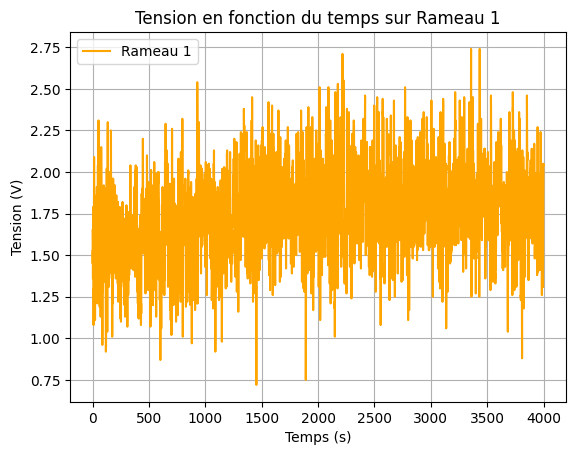
\includegraphics[width=\linewidth]{TensionEnFonctionDuTempsSecondesR1.png}
			\caption{Rameau 1 (Secondes)}
			\label{fig:r1_sec}
		\end{subfigure}
		\hfill
		\begin{subfigure}{0.48\textwidth}
			\centering
			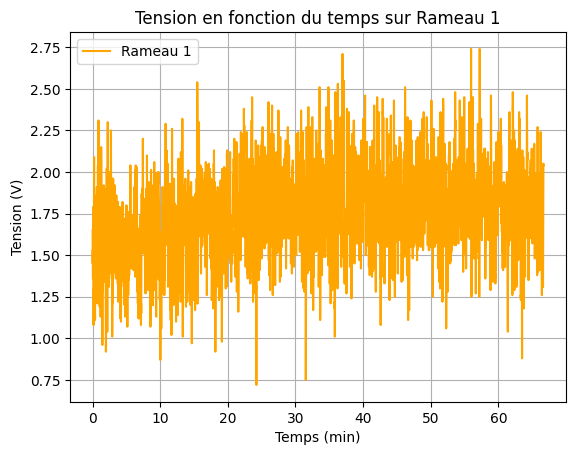
\includegraphics[width=\linewidth]{TensionEnFonctionDuTempsMinutesR1.png}
			\caption{Rameau 1 (Minutes)}
			\label{fig:r1_min}
		\end{subfigure}
		
		\vspace{0.5cm} % Espace vertical entre les deux lignes
		
		% Deuxième ligne
		\begin{subfigure}{0.48\textwidth}
			\centering
			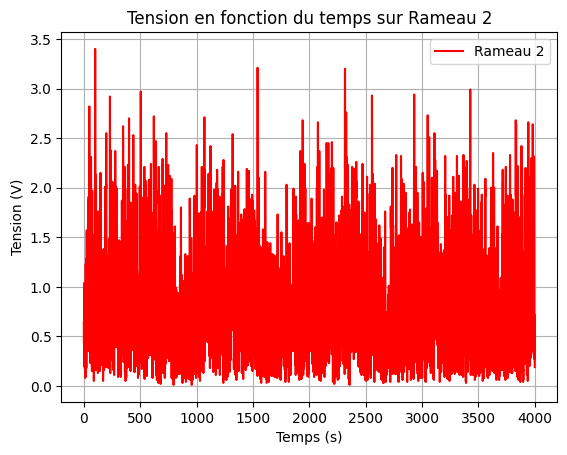
\includegraphics[width=\linewidth]{TensionEnFonctionDuTempsSecondesR2.png}
			\caption{Rameau 2 (Secondes)}
			\label{fig:r2_sec}
		\end{subfigure}
		\hfill
		\begin{subfigure}{0.48\textwidth}
			\centering
			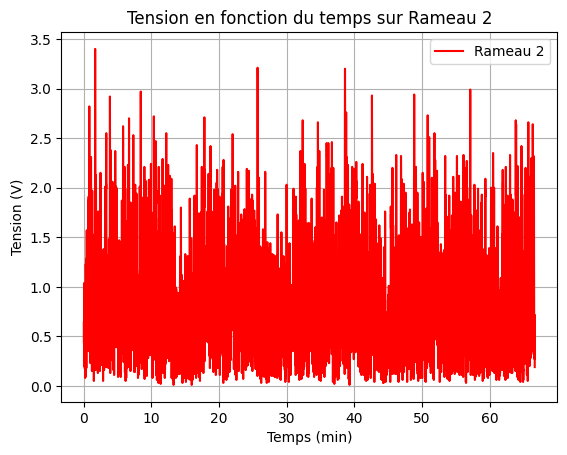
\includegraphics[width=\linewidth]{TensionEnFonctionDuTempsMinutesR2.png}
			\caption{Rameau 2 (Minutes)}
			\label{fig:r2_min}
		\end{subfigure}
		
		\caption{Évolution de la tension en fonction du temps pour les deux rameaux.}
		\label{fig:mosaique_tensions}
	\end{figure}
	
	On procède ensuite au tri des mesures en utilisant la méthode \textit{numpy.sort} et on trace les mesures triées en fonction du numéro de la mesure en figure \ref{fig:tensions_triees}
	
	\begin{figure}[H]
		\centering
		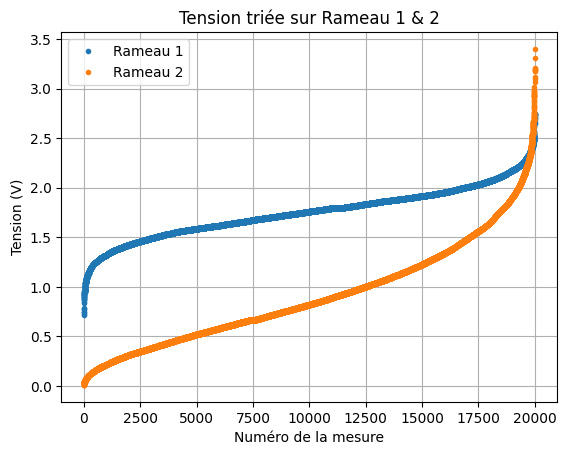
\includegraphics[width=12cm]{TensionTrieeR1R2.png}
		\caption{Tensions triées pour Rameau 1 et Rameau 2}
		\label{fig:tensions_triees}
	\end{figure}
	
	Les mesures sont discrètes, en effet, elles sont quantifiées par le système de détection qui est limité par sa mémoire. Si on utilise la fonction \textit{numpy.unique} pour déterminer le nombre de valeurs uniques de tension et on obtient 187 ce qui laisserait penser que le système est codé sur 256 bits. En zoomant sur le graphique, on voit une discontinuité entre chaque valeur de tension, et si une valeur apparaît plusieurs fois, elle s'ajoute à la suite de la valeur précédente (Voir figure \ref{fig:tensions_triees_zoom})
		
	\begin{figure}[H]
		\centering
		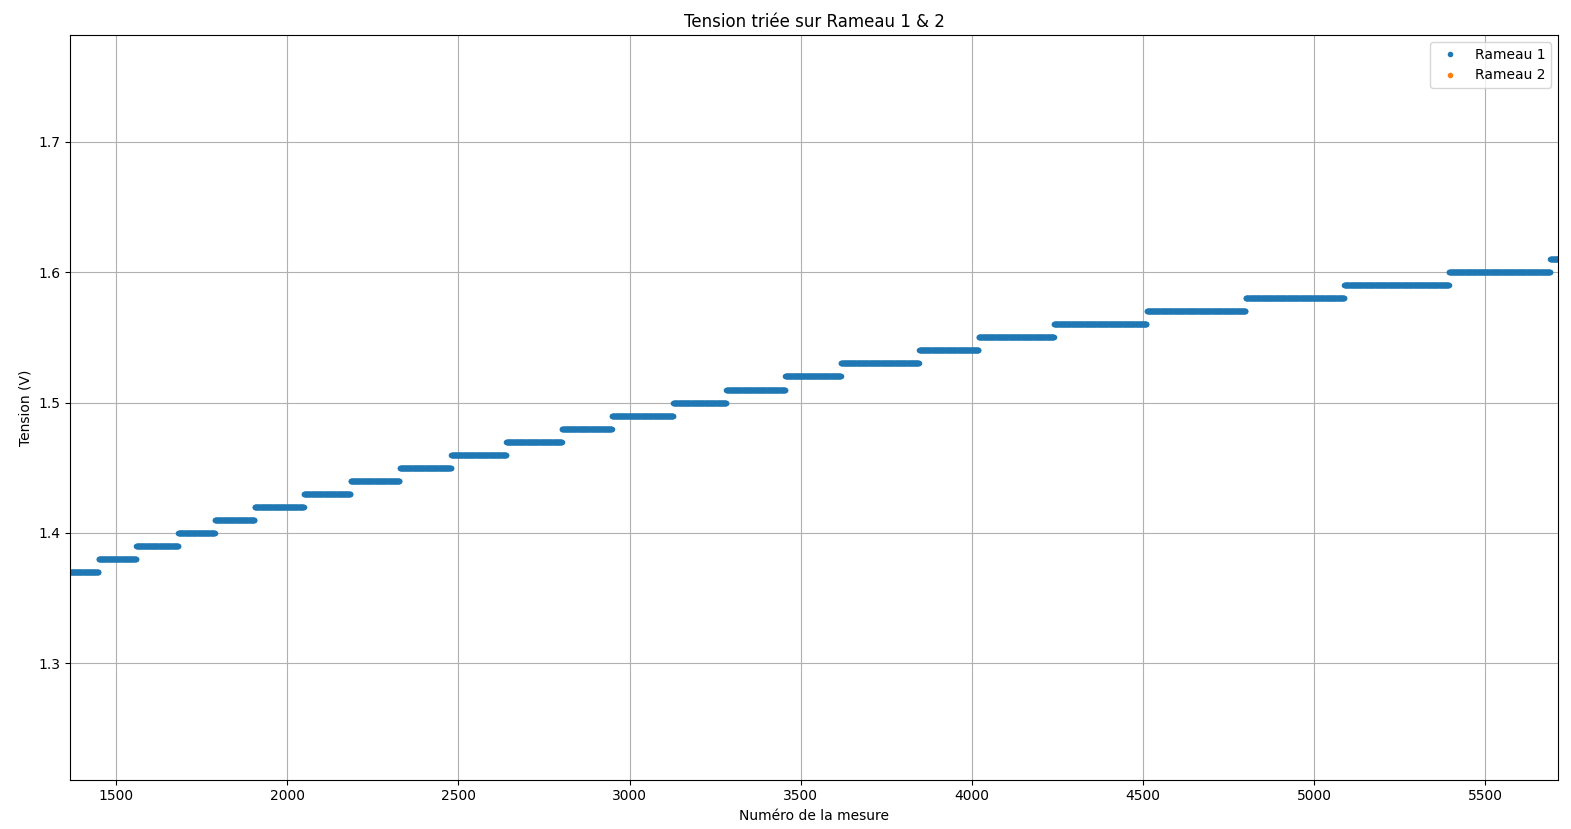
\includegraphics[width=12cm]{TensionTrieeR1R2Zoom.png}
		\caption{Zoom sur les tensions triées pour Rameau 1 et Rameau 2}
		\label{fig:tensions_triees_zoom}
	\end{figure}
	
	L'histogramme des mesures est représenté en figure \label{histogramme_R1R2}. La difficulté consiste à choisir le bon nombre de bins. Si on choisit un nombre de bins trop faible, on aura bien tous les points, mais la résolution en tension sera très faible. Si on prend un très grand nombre de bins, il y aura des intervalles vides entre certaines valeurs de tension et cela crée une grande incertitude sur la fréquence des valeurs de tension, de plus, le bruit aura plus d'impact sur la tendance globale. On choisit de prendre 25 bins.
	
	\begin{figure}[H]
		\centering
		
\includegraphics[width=12cm]{HistogrammeR1R2.png}
		\caption{Histogramme des valeurs de tensions pour Rameau 1 et Rameau 2 (25 bins)}
		\label{fig:histogramme_R1R2}
	\end{figure}
	
	La tendance de l'histogramme de Rameau 1 ressemble à une loi normale, on choisit donc d'utiliser la moyenne pour déterminer la valeur et l'écart-type pour déterminer l'incertitude sur la valeur de tension. On obtient $\mu_1 = 1.75 \ \mathrm{V}$ et $\sigma_1 =  0.26 \ V$, donc la valeur de la tension obtenue par Rameau 1 est $U_1 = 1.75 \pm 0.26 \ \mathrm{V}$.
	La mesure de Rameau 2 ne ressemble pas à une loi normale ce qui complique l'obtention de sa valeur. Les fonctions python de numpy nous permette d'obtenir le mode, la moyenne et la médiane. Cependant le mode dépend du nombre de bins et n'est donc pas fiable, la pertinence de la moyenne est discutable sur ce type de courbe. Nous choisissons donc d'utiliser la médiane: $\mu_2 = 0.82 \ \mathrm{V}$. Pour l'incertitude, nous utilisons l'écart-type même si ce n'est pas vraiment approprié pour ce type de courbe: $\sigma_2 = 0.52 \ \mathrm{V}$. Ce qui nous donne une valeur de tension pour Rameau 2 de $U_2 = 0.8 \pm 0.52 \ \mathrm{V}$.
	
	Nous obtenons une meilleure précision avec Rameau 1 et une courbe gaussienne, ce qui justifie l'utilisation de la détection synchrone.
	
	\newpage
	
	\section{Exercice 2}
	
	On souhaite déterminer expérimentalement la densité de probabilité de la distribution directe de l'erreur $\epsilon$ associée à une unique mesure, notée $f_1(\epsilon \vert I)$ pour le mode 1 et $f_2(\epsilon \vert I)$ pour le mode 2.
	Par définition, la probabilité d'obtenir un évènement dans l'intervalle [a,b] est $P(a,b) = \int_{a}^{b}p(x)dx$, où $p(x)$ est la densité de probabilité. Or une probabilité est adimensionnelle et normalisée. Donc, qualitativement:
	$$[p(x)] [x] = 1 $$ $$[p(x)] = \frac{1}{[x]}$$
	Dans notre cas, l'abscisse est la tension, donc la densité de probabilité a pour dimension le $V^{-1}$. Et donc la densité de probabilité correspond à la probabilité d'avoir une valeur de tension divisée par la largeur de la barre de l'histogramme: $$p(U) = \frac{P(U)}{\Delta x}$$. La densité de probabilité cherchée peut donc être dérivée de l'histogramme des mesures en connaissant la largeur en tension de chaque bin.
	Pour que la densité de probabilité soit normalisée, il faut que l'intégrale sur toutes les valeurs possibles fasse 1: $$\int_{-\infty}^{+\infty}p(x)dx = 1$$
	Cela signifie que l'aire sous la courbe doit valoir 1. La largeur de chaque rectangle vaut $l$ et sa hauteur vaut $h_i$. On doit donc avoir $\sum (h_i \times l) = 1$.
	Si on considère que la densité de probabilité est le comptage dans chacun des intervalles de l'histogramme, divisé par le nombre total des mesures que multiplie la largeur $l$ des intervalles, alors: $h_i = \frac{c_i}{n \times l}$
	On peut vérifier si cette expression vérifie la condition de normalisation: $$\sum (h_i \times l) = \sum (\frac{c_i}{n \times l} \times l) = \sum P_i = 1$$
	Ainsi cette expression de la densité de probabilité $p(U)$ vérifie la condition de normalisation. On trace la densité de probabilité d'obtenir chaque valeur de tension pour Rameau 1 en figure \ref{fig:densite_R1}
	
	\begin{figure}[H]
		\centering
		
\includegraphics[width=12cm]{DensiteR1.png}
		\caption{Densité de probabilité d'obtenir une valeur de tension pour Rameau 1}
		\label{fig:densite_R1}
	\end{figure}
	
	On constate que cette densité de probabilité peut être supérieure à 1, ça ne pose pas de problème car elle est normalisée par la largeur de chaque barre d'histogramme, or cette valeur peut être inférieure à 1.
\end{document}	